The dual perspective offered by spectral graph theory for studying the dynamics of Markov chains is exploited in this chapter for options discovery. As opposed to other similar algorithms \parencite{Menache2002, Mannor2004, Mathew2012, Bouvrie2012}, the problem of discovering and constructing options in continuous state space is tackled. This setting brings along additional challenges in terms of computational efficiency, function approximation and graph representation.

The main distinction between the control techniques of RL and those of the more traditional stochastic dynamic programming approach is that the latter assumes some knowledge of the transition and reward probabilities. Therefore, the graph Laplacian underlying an MDP  cannot be assumed to be available  under the RL setting. By sampling a large number of state-action transitions, the dynamics could certainly be recovered in the limit. The curse of dimensionality would however quickly render this approach hopeless.

One way to address this problem is by building a \textit{proximity graph}
over sampled states. While such a representation is not faithful to the Markov chain induced by some optimal policy, useful geometrical properties can still be inferred by resorting to the random walk process.  This reduction is not without consequence as the precious optimality-preserving transitions of $\mathbf{P}_\pi$ are completely ignored. The random walk graph Laplacian can capture relevant geometrical features of the state space, which in certain environments,  also reflect optimal structures of the solution space. \cite{Mahadevan2007} also had recourse to the same strategy but argued for its merits in transfer learning.

\section{Graph Construction}
\label{sec:proximitygraphs}

When dealing with a discrete state space, the task of estimating the state-transition graph is much easier than with its  continuous counterpart. It suffice indeed to collect sample trajectories and setting graph edges between any two temporally successive states. In the continuous case, temporal ordering can be enough to reconstruct a single geodesic from a trajectory but merging them to form a graph is problematic. Furthermore, with a countably infinity state space, the probability of encountering exactly the same state twice is infinitely small.  In machine learning, a common approach for estimating the low-dimensional manifold assumed to underly a set of points consists in building a \termidx{proximity graph}. The same technique is adopted in this work for estimating the random walk Laplacian.

Proximity graphs arise from the general problem of extracting geometrical structure from a set of points in the plane. In machine learning, they are commonly found in non-linear dimensionality reduction techniques \parencite{Tenenbaum2000, Roweis2000}, clustering \parencite{Luxburg2007} or non-parametric classification \parencite{Toussaint2012}. Under the manifold assumption, in a \textit{small enough} region around a point, the topological space is assimilable to the Euclidean space. Edges in a proximity graph then capture the notion of distance in this neighbourhood. 

\subsection{Empty Region Graphs}

\begin{defn}
The circle passing through all three vertices of a triangle is called the \termidx{circumcircle of a triangle}.
\end{defn}

\begin{defn}
The \termidx{Delaunay Triangulation} (DT) of a set $V$ is the dual of the \termidx{Voronoi diagram} decomposing $\mathbb{R}^d$ into $|V|$ \textit{cells}. The Delaunay Triangulation is obtained by setting edges between any two adjacent cells in the Voronoi diagram. The DT also has the property that no point can be found in the circumcircle of any triangle. 
\end{defn}

\begin{figure}
\centering
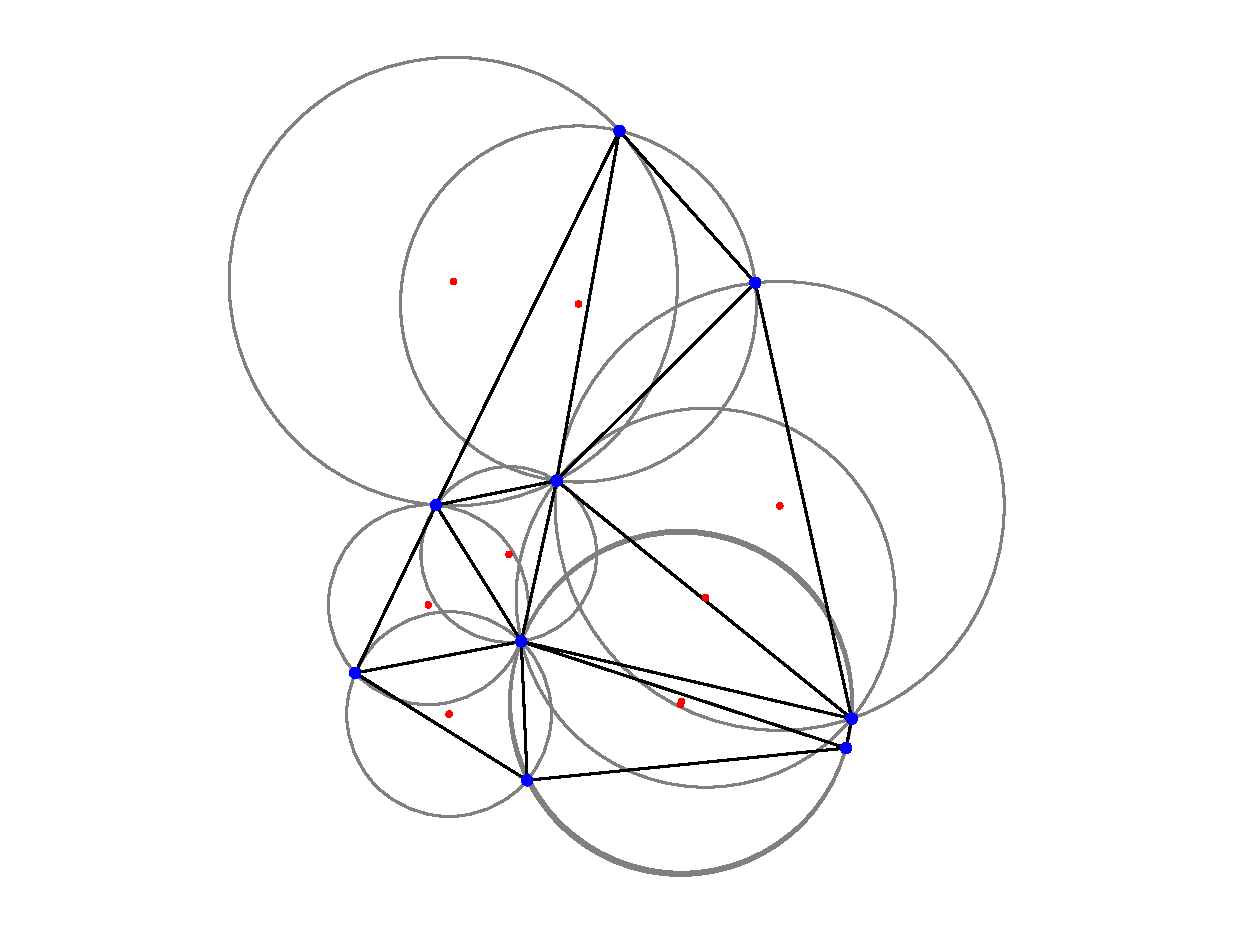
\includegraphics[scale=0.5]{fig/Delaunay-circle.eps}
\caption{The Delaunay triangulation of a set of points in the plane. The red points indicate the circumcenters. It can be seen that no vertex is within the circumcircle of some triangle.}
\label{fig:delaunay}
\end{figure}

From a practical point of view, the Delaunay triangulation offers the advantage of
producing connected graphs. However, it only comes at the cost of having a much larger edge set. In $\mathbb{R}^d where \geq 3$, the number of triangles in the Delaunay graph is known to be $\Omega(n^{\lceil\frac{d}{2} \rceil})$. Furthermore, the worst case complexity for computing it in $d \geq 3$ is $\mathcal{O}(n^{\lceil\frac{d}{2} +1 \rceil})$ using the gift-wrapping algorithm \parencite{Fortune1997}.

\begin{defn}
Let $B(x, r)$ denote the sphere or radius $r$ centered at $x$ and $\delta(p,q)$ be the distance between two points $p$ and $q$ (figure \ref{fig:erg-construct}). Let the neighborhood of two points be defined by $\Pi_{p,q} = B(\frac{p+q}{2}, \frac{\delta(p, q)}{2})$. The \termidx{Grabriel graph} (GG) of a set of vertices $V$ is such that for all edges $(p, q) \in E$  the space within $\Pi_{p,q}$ is empty. That is, $\Pi_{p,q} \cap V = \varnothing$
\end{defn}

\begin{figure}[ht]
\centering
\subbottom[GG]{%
\documentclass{standalone}
\usepackage{tikz}
\begin{document}
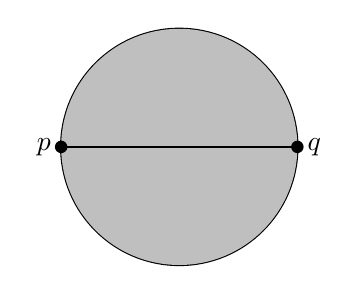
\begin{tikzpicture}[thick, scale=0.75]
\draw (0,0) circle (2cm);
\fill [gray!50] (0,0) circle (2cm);

\path (-2, 0) coordinate [label= left:$p$] (p);
\path (2,0) coordinate  [label= right:$q$] (q);
\draw (p) -- (q);
\fill [black] (p) circle (3pt);
\fill [black] (q) circle (3pt);
\end{tikzpicture}
\end{document}}
\subbottom[RNG]{
\documentclass{standalone}
\usepackage{tikz}
\begin{document}
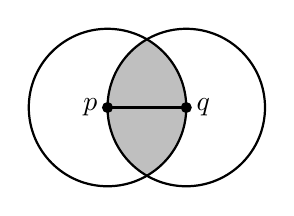
\begin{tikzpicture}[thick, scale=1.0]
\begin{scope}
\clip (-0.5,0) circle (1cm);
\clip (0.5,0) circle (1cm);
\fill[color=gray!50] (-1,1) rectangle (1,-1);
\end{scope}

\draw (-0.5,0) circle (1cm);
\draw (0.5,0) circle (1cm);
    
\path (-0.5, 0) coordinate [label= left:$p$] (p);
\path (0.5,0) coordinate  [label= right:$q$] (q);
\draw (p) -- (q);
    
\fill [black] (p) circle (2pt);
\fill [black] (q) circle (2pt);
\end{tikzpicture}
\end{document}}
\caption{Empty regions of the GG and RNG. The shaded area represents the empty region.}
\label{fig:erg-construct}
\end{figure}

The Gabriel graph was introduced in \cite{Gabriel1969} for the analysis of geographic data. In the worst case, the GG of a set of points yields $\Omega(n^2)$ edges \parencite{Toussaint1992}. The expected number of edges of the GG was also studied by \cite{Devroye1988} and shown to be order of $2^{d-1}n$ for most probability densities. In $d$ dimensional Euclidean space, the trivial brute-force algorithm in $\mathcal{O}(dn^3)$ time complexity is the only one known to date \parencite{Toussaint2012}.

\begin{defn}
The intersection of the two balls centered at $p$ and $q$ and of radius $\delta(p,q)$ respectively is called a \textit{lune} (figure \ref{fig:erg-construct}); $\Lambda_{p,q} = B(p, \delta(p,q)) \cap B(q, \delta(p,q))$. The \termidx{Relative Neighborhood Graph} (RNG) is the graph for which the set of edges $E$ is such that $(p,q) \in E 	\text{ if and only if } \Lambda_{p,q} \cap V = \varnothing$ 
\end{defn}

The Relative Neighborhood graph was introduced by \cite{Toussaint1980} and studied for its ability to capture perceptually meaningful regularities. It was also shown that in the Euclidean plane, the minimum spanning tree (MST) is a subgraph of the RNG which in turns is contained in the DT. In $\mathbb{R}^d, d > 3$, the maximum number of edges in the RNG is $\Omega(n^2)$ \parencite{Toussaint1992} and the brute-force algorithm for computing it is $\mathcal{O}(n^3)$ \parencite{Toussaint1980}.

\begin{defn}
The Euclidean Minimum Spanning Tree (EMST) is the minimum tree that connects every vertices with minimum weights sum. The EMST is a subgraph of the Delaunay triangulation.
\end{defn}

The fastest algorithm for computing the EMST was recently obtained by \cite{March2010} and appears to be approximately $\mathcal{O}(n \log n)$ even in $\mathbb{R}^d$.
 
 \begin{figure}
  \centering
    \subbottom[Delaunay triangulation]{%
    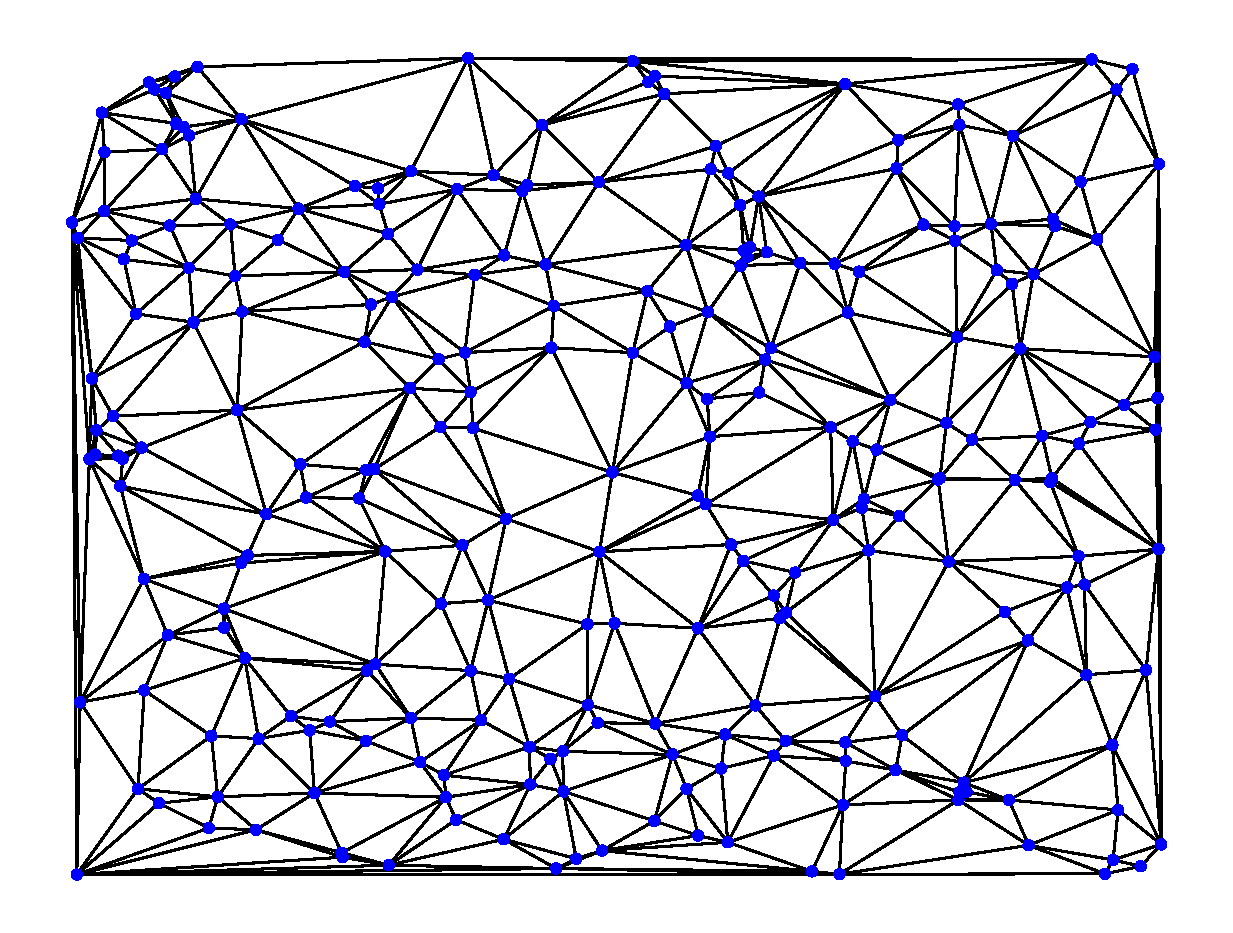
\includegraphics[width=0.45\linewidth]{fig/Delaunay-graph.eps}}
    \subbottom[Gabriel Graph]{%
    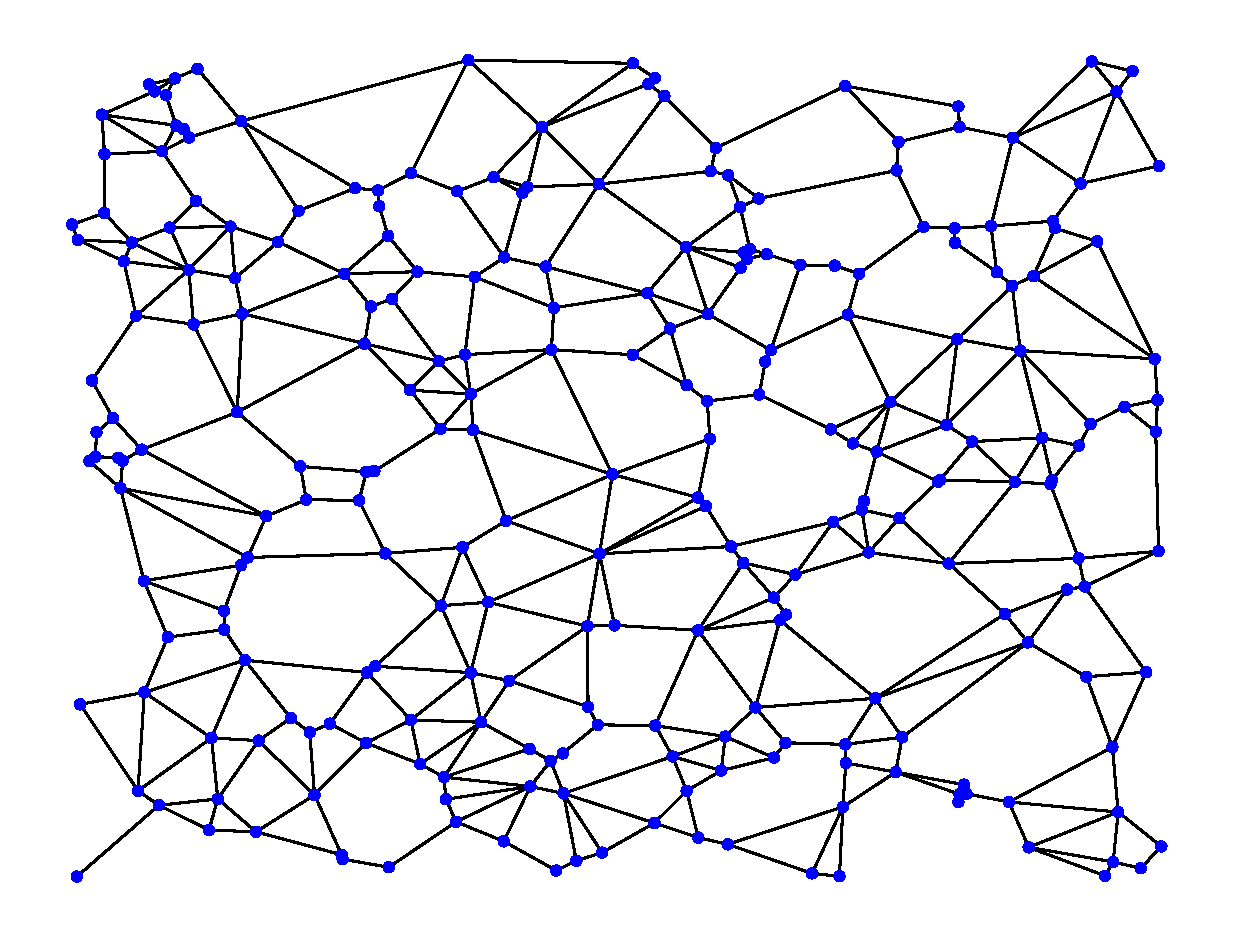
\includegraphics[width=0.45\linewidth]{fig/Gabriel-graph.eps}}
    \subbottom[RNG]{%
    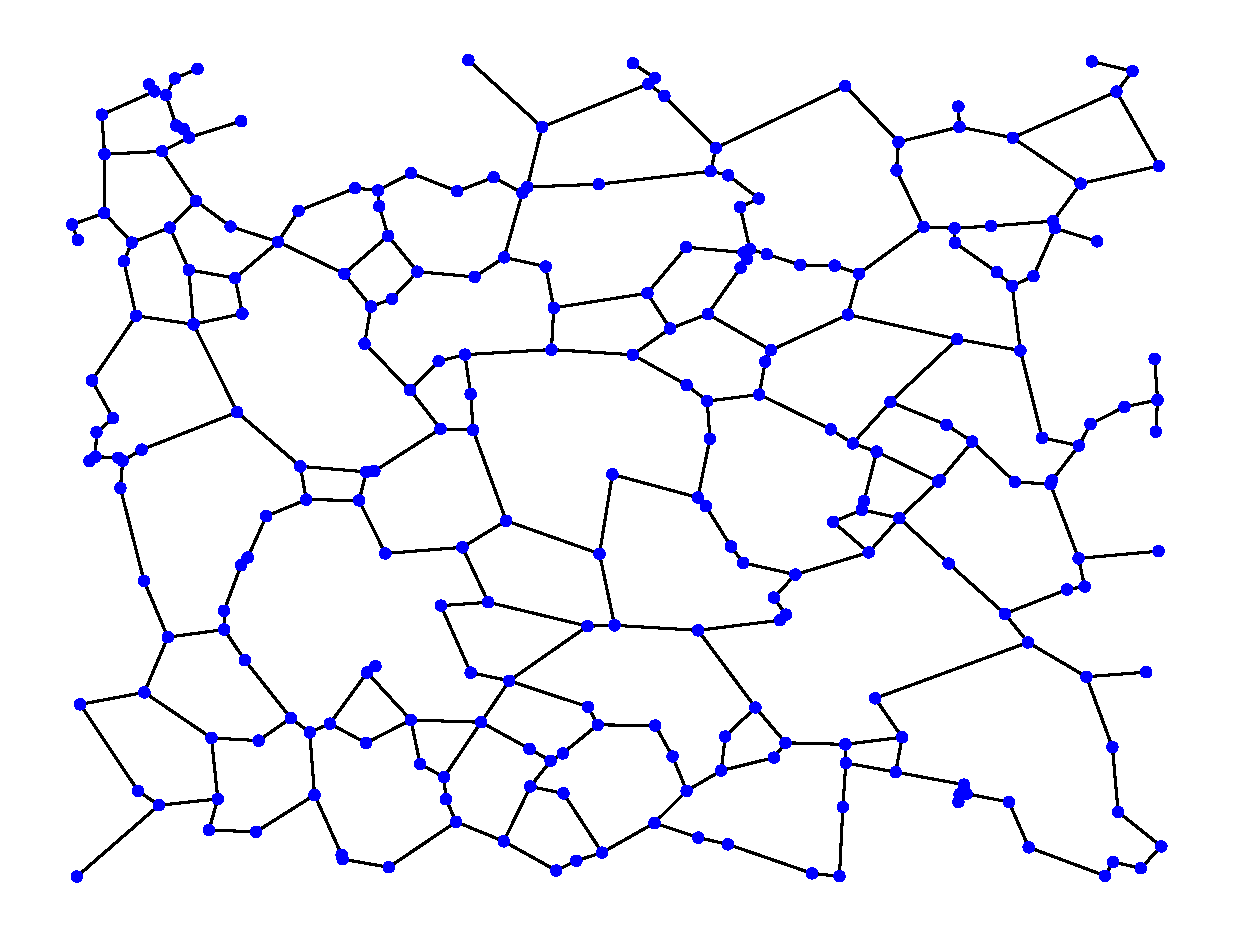
\includegraphics[width=0.45\linewidth]{fig/RNG-graph.eps}}
    \subbottom[EMST]{%
    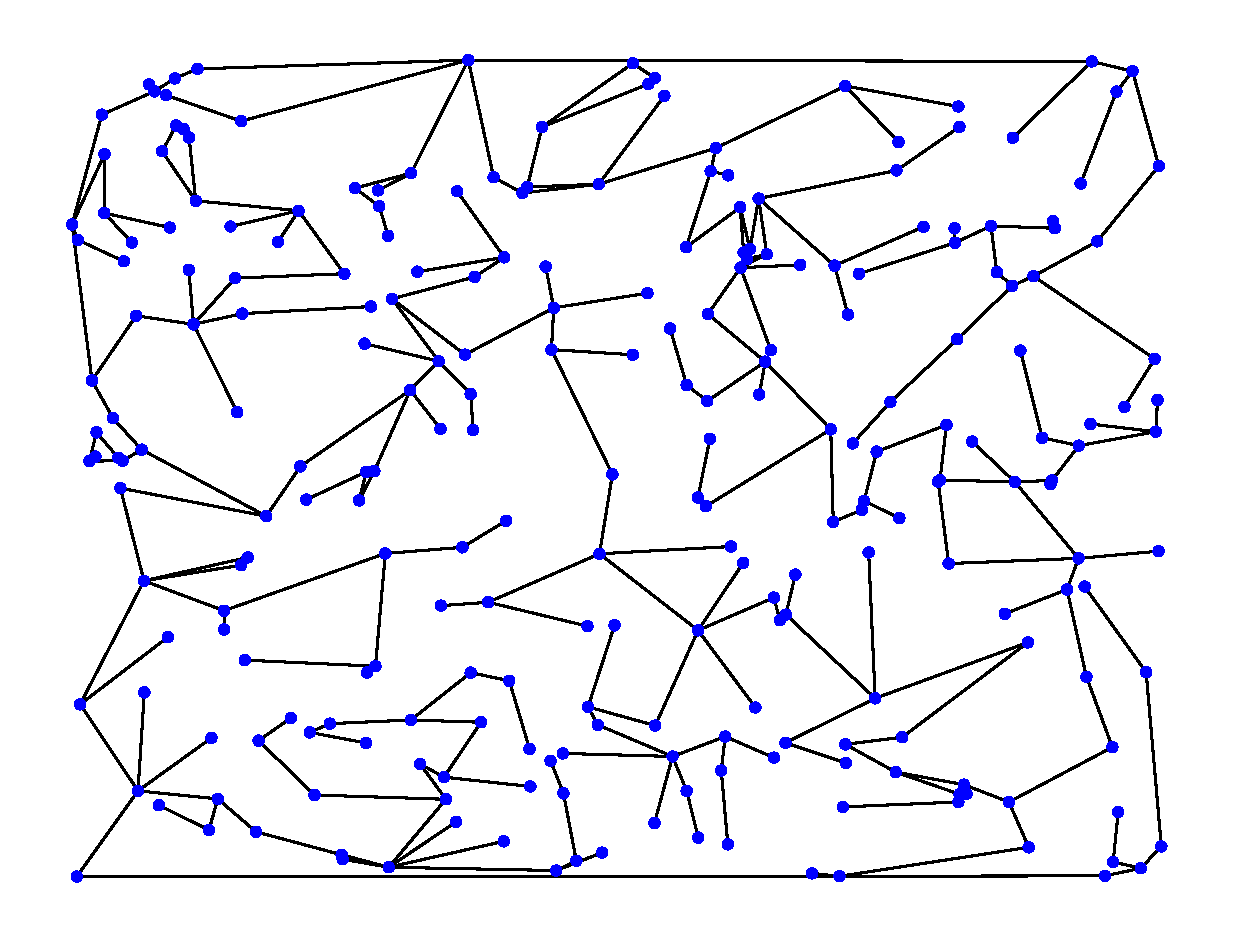
\includegraphics[width=0.45\linewidth]{fig/EMST-graph.eps}}    
    \caption{Empty region graphs, ordered according to $EMST(V) \subseteq RNG(V) \subseteq GG(V) \subseteq DT(V)$. A set of 250 points were drawn uniformly at random in $\mathbb{R}^2$}
\end{figure}

\subsection{Nearest Neighbor Graphs}

While the empty region graphs presented in the last section are geometrically appealing, their density (exponential for the GG) is problematic. Furthermore, the computational cost for obtaining them is prohibitively expensive for the general large scale problems envisioned in this thesis. The class of nearest neighbor graphs tends to be a good replacement against these issues and have a long history in spectral clustering \parencite{Luxburg2007}.

\begin{defn}
The \termidx{Nearest Neighbor Graph} (NNG) is a directed graph connecting vertex $p$ to $q$ if $q$ is the nearest neighbor of $p$.
\end{defn}

The nearest neighbor relation is not symmetric and thus forgo a definition of NNG as an undirected graph. When admitting $k$ nearest neighbors, the concept can be generalized to the K-NNG \parencite{Miller1997} and the NNG appears to be only a special case where $k=1$.

\begin{defn}
The \termidx{Symmetric K-Nearest Neighbor Graph} (K-NNG) is graph in which an edge connects vertex $p$ to $q$ only if $q$ is among the $k$ nearest neighbors of $p$. Let $N_k(p)$ denote the set of $k$ points closest to $p$, the edge set is defined as
\begin{equation}
E = \{ (p, q) : p \in N_k(q) \textbf{ or } q \in N_k(p) \}
\end{equation}
\end{defn}

\begin{defn}
The \termidx{Mutual K-Nearest Neighbor Graph} (K-NNG) is graph for which an edge connects vertex $p$ and $q$ only if $q$ is among the $k$ nearest neighbors of $p$ and similarly for $q$ in the other direction. That is, 
\begin{equation}
E = \{ (p, q) : p \in N_k(q) \textbf{ and } q \in N_k(p) \}
\end{equation}
\end{defn}

\begin{defn}
The \termidx{$\epsilon$-Graph} is the graph connecting vertex $p$ and $q$ only if $q$ is within a ball of radius $\epsilon$ centered at $p$. That is, 
\begin{equation}
E = \{ (p, q) : \delta(p, q) < \epsilon \}
\end{equation}
\end{defn}

 \begin{figure}[ht]
  \centering   
    \subbottom[Input points]{%
    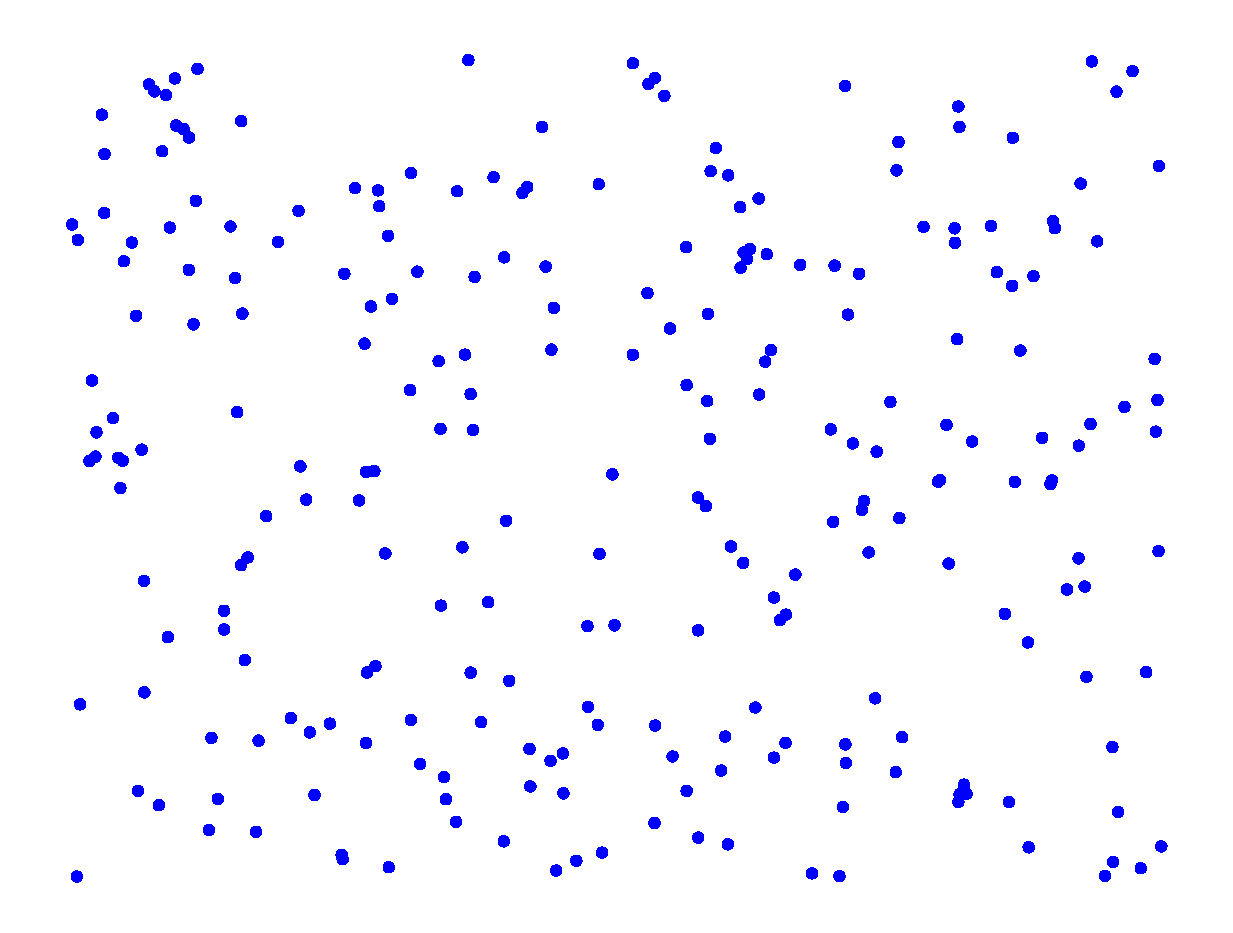
\includegraphics[width=0.45\linewidth]{fig/Points-graph.eps}}
    \subbottom[Symmetric Graph]{%
    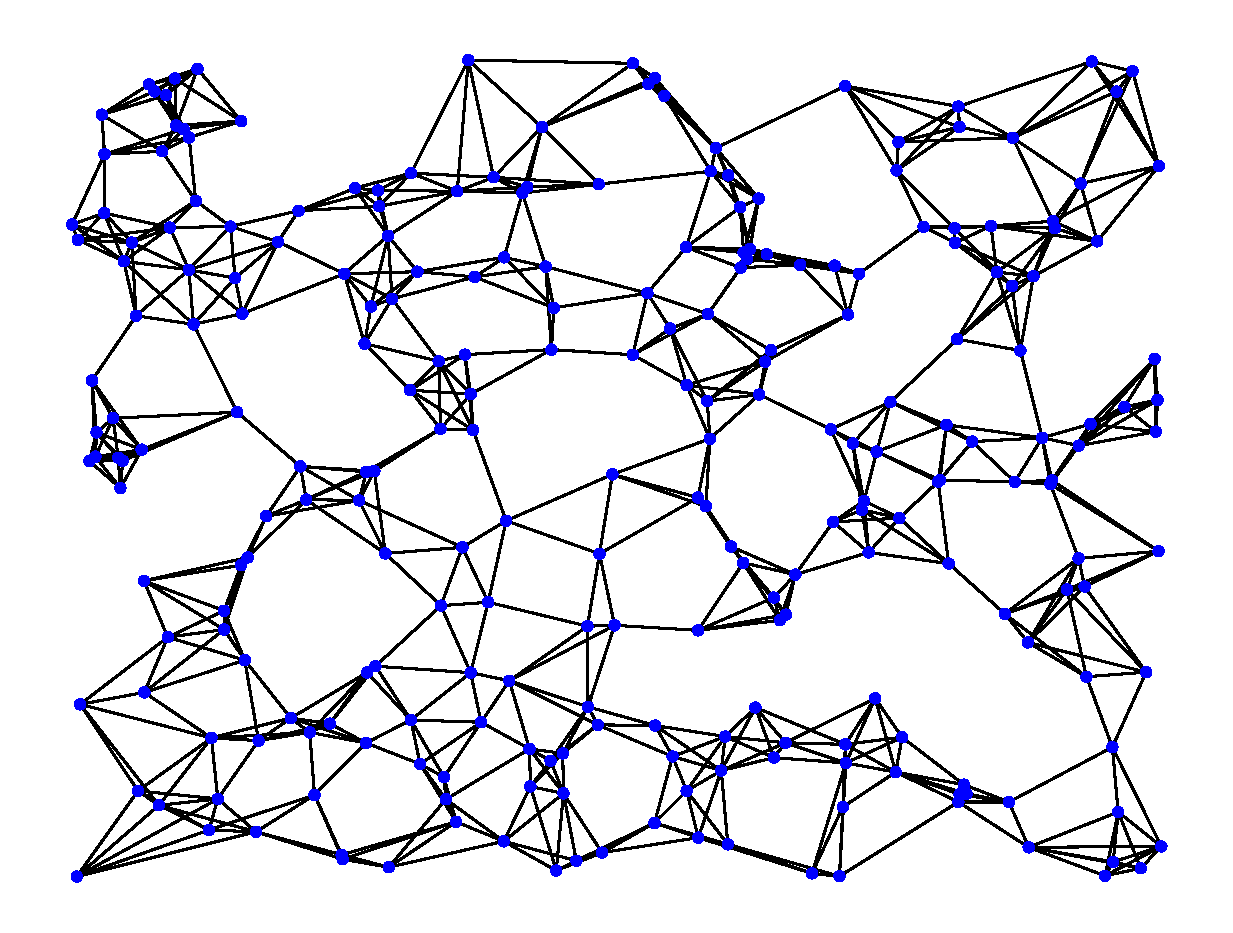
\includegraphics[width=0.45\linewidth]{fig/Symmetric-graph.eps}}
    \subbottom[Mutual Graph]{%
    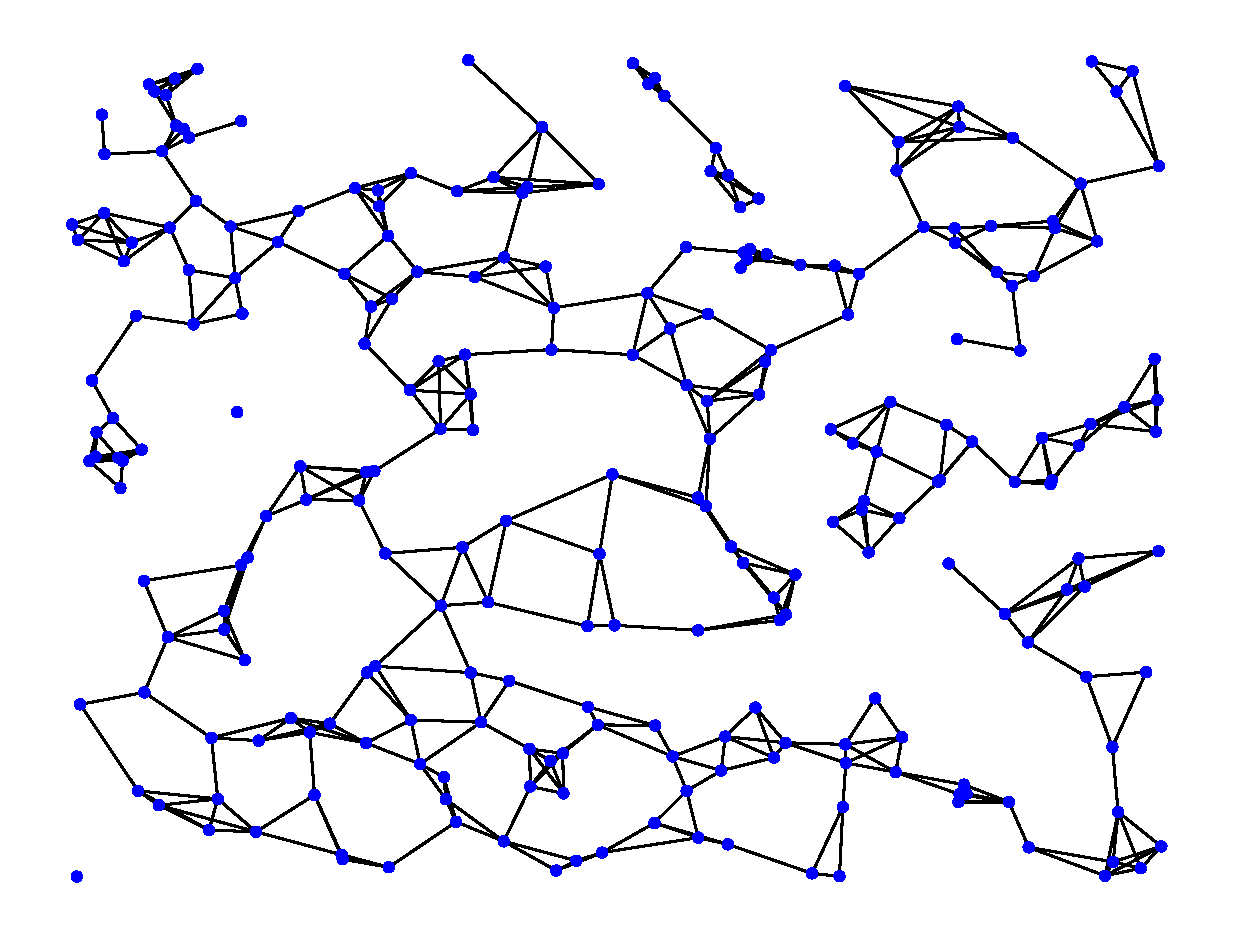
\includegraphics[width=0.45\linewidth]{fig/Mutual-graph.eps}}
    \subbottom[$\epsilon$-graph]{%
    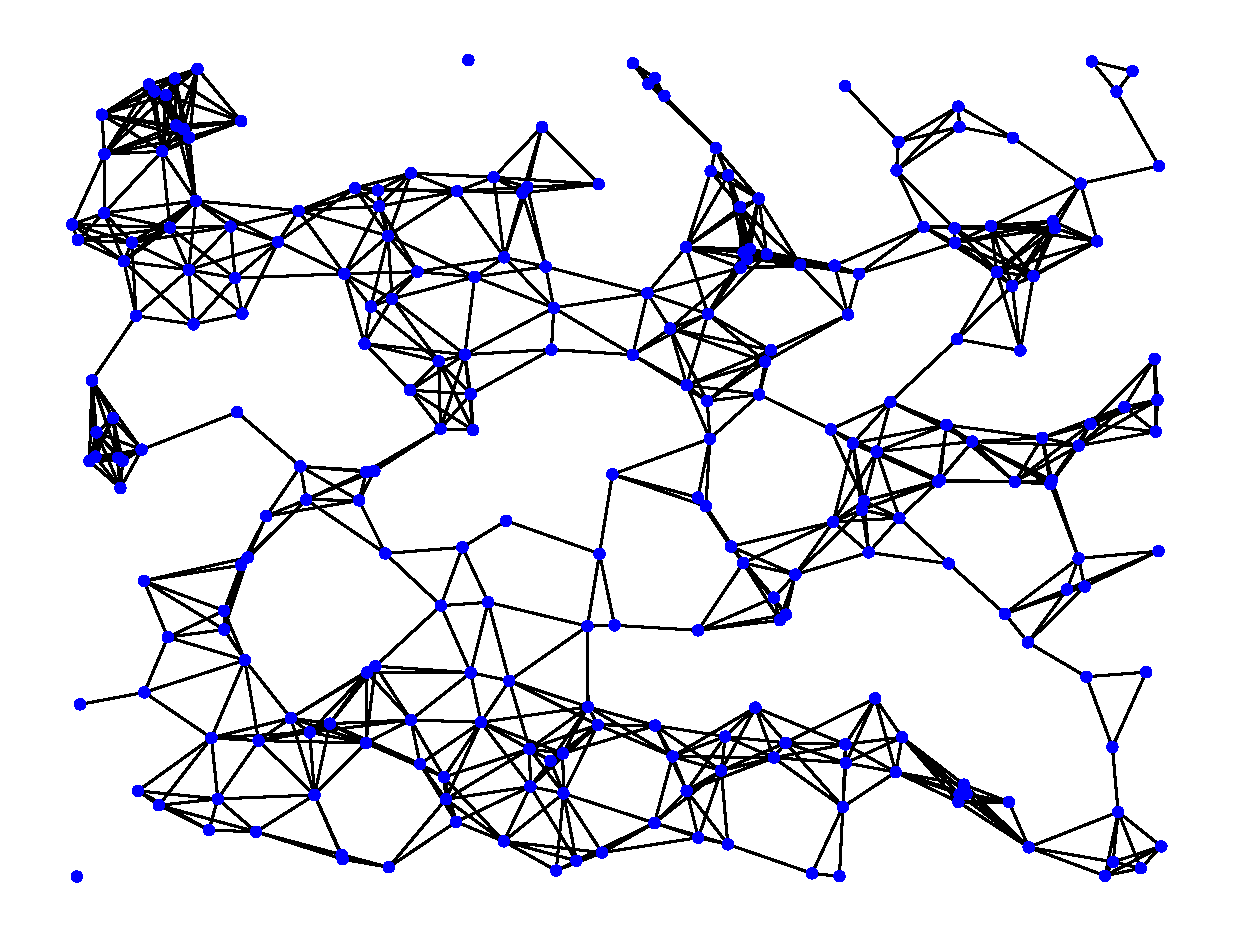
\includegraphics[width=0.45\linewidth]{fig/Epsilon-graph.eps}}   
  \caption{K-NN Graphs. The number of nearest neighbors was set to $k=5$ for the first two examples while $\epsilon$ was set to $0.01$ for the last.}
  \label{fig:knn-graphs}
\end{figure}

The choice of an appropriate radius for the $\epsilon$-graph tends to be difficult to obtain in practice. Furthermore, if the sampled data exhibit varying densities, a fixed value for $\epsilon$ would do poorly and potentially result in a disconnected graph. The mutual graph is usually sparser and can better function over constant densities. It however also leads more easily to  disconnected graphs as shown in figure \ref{fig:knn-graphs}. Finally, the symmetric graph better handles data at different scales but produces more edges.  

K-NN graphs can be implemented effectively using a KD-Tree \parencite{Friedman1977}
structure in low dimensions but otherwise suffers from the curse of dimensionality.
When allowing for approximate neighbors, very efficient algorithms have recently
been proposed to solve this problem based on the concept of \textit{locality-sensitive
hashing} \parencite{Andoni2008}. As opposed to the KD-Tree approach, these algorithms perform
efficiently in high dimensional spaces. 

\section{Graph Clustering}
Chapter \ref{chap:dynamics} shows how the spectral properties of the graph Laplacian can reveal the clusters structure. In general, computing the eigenvectors of dense matrices is $\mathbb{O}(n^3)$, making the \textsc{NCut} criterion difficult to apply over large state spaces. The community detection algorithm of \cite{Newman2006}, the archetypical spectral clustering of \cite{Ng2001}, or the \textsc{PCCA+} algorithm of \cite{Deuflhard2005} all exhibit the same running time.

The random walk perspective of graph partitioning is taken in the \textsc{Walktrap} algorithm by \cite{Pons2005} to reduce the time complexity usually associated with the other class of algorithms. The intuition underlying this algorithm is that of a random walker visiting the graph and spending more time -- getting \textit{trapped} -- into densely connected regions and on rare occasions, jump to a different set of vertices.

This probabilistic interpretation of graph partitioning had already been exploited thoroughly in the literature on NCD systems (section \ref{sec:ndmc}) and highlighted by \cite{Shi2001}, a corner stone for spectral clustering techniques in machine learning. The contribution of \textsc{Walktrap} was to show how a probabilistic distance measure can be defined between vertices and used to obtain clusters using a fast agglomerative method.

Given the random walk transition matrix $\mathbf{P}$, the distance
measure between two vertices is defined as 
\begin{equation}
r_{ij} = \sqrt{\sum_{k=1}^n \frac{P_{ik}^t - P_{jk}^t}{d_k}} = \| D^{-1/2}
[\mathbf{P}^t]_i - D^{-1/2} [\mathbf{P}^t]_j \|_2
\label{eq:diffusion-distance}
\end{equation}

where $\| \cdot \|_2$ is the Euclidean norm and $[\mathbf{P}]^t_i$ is the
ith row of matrix $\mathbf{P}$. It appears that the same measure was
presented under the name of \textit{diffusion distance} in the same year
by \cite{Nadler2005}. Both papers also relates it to the spectrum of $\mathbf{P}$ by
showing that it amounts to explicitly computing the embedding and taking the Euclidean
distance in that space (what \cite{Nadler2005} calls the \textit{diffusion space}).
 
Intuitively, the diffusion distance measures the $L^2$ distance between two probability
distributions. The vector $[P^t]_i$ contains the probabilities of starting from vertex $i$
and reaching any other vertex $j$ in $t$ steps, taking into account all possible paths 
between them. For two vertices within a community, their probability vector are
expected to be very close as they are both likely to reach the other vertices using the
same paths. However, two vertices in different communities \textit{see} very different
sets of vertices under $t$ steps and their distance thus must be larger. \cite{Nadler2005} refers to this notion of distance as the \textit{dynamical proximity} since it depends on the dynamics of the random walk over the graph. Varying the number of steps $t$ also has for effect to expose the dynamics at different scales. In dense graphs, fewer steps are required to cover a larger portion of the graph. On the other hand, in sparser graphs larger values for $t$ would not impact as much the locality of the vertices being visited. 

The distance measure defined in equation \ref{eq:diffusion-distance} yet remains to be incorporated into a clustering scheme. Ward's agglomerative method \parencite{Ward1963} is used in \textsc{Walktrap} to obtain sets of vertices which are as similar as possible with respect to this measure. Initially, the algorithm starts with $|V|$ singleton partitions.  At each iteration, communities are merged in a pairwise manner and the distances for the new partitions are updated. The notion of distance between communities is a straightforward extension of equation \ref{eq:diffusion-distance} and expresses the probability of going from a given community $C$ to any vertex $j$ in $t$ steps.  \label{sec:walktrap}
\begin{align}
P^t_{Cj} &= \frac{1}{|C|} \sum_{i \in C} P^t_{ij} \\
r_{C_1, C_2} &= \| D^{-1/2} P_{C_1 \bullet}^t - D^{-1/2} P_{C_2 \bullet}^t\|
\end{align}

The vectors $P^t_{C\bullet}$ are thus probability distributions over the graph expressing the probabilities of choosing uniformly a vertex from $C$ and reaching some other vertex $j$ under $t$ steps. What makes Ward's algorithm efficient in this setting is that the distances after merging can be updated efficiently. Each distance computation requires $\mathcal{O}(n)$ and an upper bound is given as a function of the height of the dendogram. The number of distance computations is $\mathcal{O}(mn(H + t))$ \parencite{Pons2005} (theorem 7). For sparse graphs where the number of edges $m = |V|$ and the height of the dendogram is $\mathcal{O}(\log n)$, the worst case complexity then becomes $\mathcal{O}(n^2 \log n)$. In the general case, the complexity is otherwise $\mathcal{O}(mn^2)$. 

\section{Algorithm}

A fast method for discovering and learning subgoal options is presented in algorithm \ref{alg:knnoptions}. For each option, a terminal subgoal value (pseudo-reward) $g$ is overlaid to the underlying reward function of the base MDP. The type of features or optimal control algorithm is left unspecified. In the experiments presented in the next chapter, Fourier features and SARSA were used. The Least-Square Policy Iteration (LSPI) \parencite{Lagoudakis2003} algorithm could equally do well and make efficient use of the batch data collected in the first step. In order to make the algorithm capable of handling large state spaces, the \textsc{Walktrap} algorithm is used to discover dynamically stable regions of the state space from the random walk process. 

\begin{algorithm}
\DontPrintSemicolon
\KwData{An environment from which to collect experience, terminal subgoal reward $R_{subgoal}$, number of random walk steps $t$, number of nearest neighbors $k$}
\KwResult{A set of options}
\SetKwData{Dataset}{dataset}
\SetKwData{Index}{index}
\SetKwData{Edges}{edges}
\SetKwData{Vertices}{vertices}
\SetKwFunction{Walktrap}{Walktrap}
\SetKwData{g}{g}
\SetKwFunction{Graph}{Graph}
\SetKwData{Communities}{communities}
\SetKwFunction{Option}{Option}
\SetKwData{Options}{options}
\SetKwData{Subgoals}{subgoals}
\SetKwFunction{Boundary}{$\partial$}
\SetKwFunction{LearnMDP}{LearnSubgoalMDP}
\;

\textbf{1. Acquire experience} \;
\Dataset $\leftarrow$ collect samples of experience $\{(x_t, a_t, x_{t+1}, r_{t})\}$ through some fixed policy. A random walk process can be used if the optimal policy is not known. \;
\Dataset $\leftarrow$ optionally subsample the dataset uniformly at random if too large\;
\Index $\leftarrow$ build an approximate nearest neighbor index over the sampled states\;
\;
\textbf{2. Build the symmetric K-NN graph}\;
\Vertices $\leftarrow $ set of sampled $x_t$ in \Dataset \;
\Edges $\leftarrow \varnothing$\;
\ForEach{state $x$ in dataset} {
knn $\leftarrow$ query the $k$ nearest neighbors of $x$\;
  \ForEach{nearest neighbor $nn$ \KwSty{in} knn} {
    \Edges $\leftarrow$ \Edges $\cup \; (x, nn)$\;
  }
}
\;
\textbf{3. Discover and learn options} \;
\Communities $\leftarrow$ \Walktrap{\Graph{\Vertices, \Edges}, t} \;
\Options $\leftarrow \varnothing$ \;
\ForEach{community c \KwSty{in} \Communities} {
  $\mathcal{I} \leftarrow c$\;
  \Subgoals $\leftarrow \partial(c)$\;
  $\beta \leftarrow \indicator_{\Subgoals}$ \;
   $\g \leftarrow \indicator_{\Subgoals}\cdot R_{subgoal}$\;
   $\pi \leftarrow$ \LearnMDP{\g} \;
   \Options $\leftarrow$ \Options $\; \cup \;$ \Option{$\mathcal{I}$, $\beta$, $\pi$} \;
}
\Return \Options
\caption{\textsc{Bottleneck-Options} construction algorithm}
\label{alg:knnoptions}
\end{algorithm}

The symmetric K-NN proximity graph construction was retained for its computational efficiency, better adaptation across different scales and sparsity. In the spectral clustering literature the problem of obtaining a similarity graph is sometimes neglected by simply assuming a complete graph with $n^2$ edges. Such a dense representation however quickly leads to poor computational performance. K-Nearest Neighbor graphs are also used for spectral clustering and their empirical properties are  discussed in \cite{Luxburg2007}. The family of empty regions graphs consisting of the beta-skeleton graph, GG and RNG was also investigated in \cite{Correa2012}. The use of EMST graphs was ruled out in this algorithm because of its extreme sparsity. It is worth nothing however that \cite{Carreira2004} experimented with ensembles of \textit{perturbed} EMST. The resulting denser combined graph was reported to perform well for clustering.

In practice, the choice of $k$ dramatically impacts the clustering. It is often desirable to simply settle on a value which leads to a connected graph. Little is known in the spectral clustering literature about the effect of this parameter and even less about the general problem of choosing an suitable proximity graph construct. \cite{Maier2008} provides some theoretical results about the convergence of graph clustering as a function of $k$ but fail to provide practical guidelines. 

\subsection{Initiation and Termination in Continuous Space}
\label{sec:knnoptions}
When applying algorithm \ref{alg:knnoptions} in continuous state spaces, the definition of the initiation and termination components needs to be generalized over regions rather than only discrete states. Having already constructed a nearest neighbor index for  the proximity graph, an efficient solution is also to use it in the definition of the termination function as

\begin{equation}
\beta(x) = 
\begin{cases}
1 & \text{if } N_1(x) \in C_x\\
0 & \text{otherwise}
\end{cases}
\end{equation}

where $N_1(x)$ is the first NN of $x$ and $C_x$ stands for the community to which $x$ belongs to. For better robustness against noise, the majority vote among $k$ nearest neighbors can be taken.

Membership to the initiation set can be determined by a logical negation of $\beta$. Let $C$ be the community associated with the initiation set of an option, a membership query consists in
\begin{equation}
N_1(x) \in C \Rightarrow x \in C  \\
\end{equation}

Once again, majority voting can be used to reduce the effect of noise. 
